\problemname{Average Rank}

The National Weekly Escape Room Challenge (NWERC) is a long-running competition held in Eindhoven.
Every week a new escape room is presented, and anyone who completes it in their first attempt gains one point.

At the end of each week, competitors are ranked by the total number of points accumulated so far, highest first. In case of a
tie, they share the same rank. In other words, the rank of a competitor is one more than the number of people
with a strictly larger number of points.

\begin{figure}[h!]
  \centering
  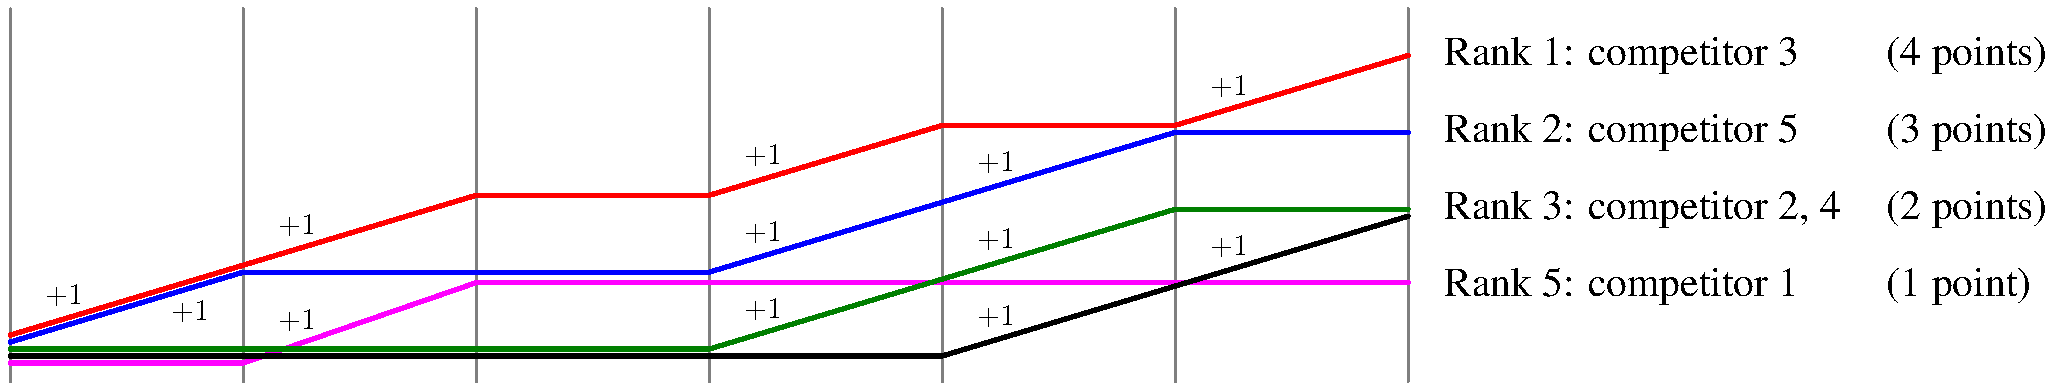
\includegraphics[width=1.0\textwidth]{ranks}
  \caption{Illustration of Sample Input 3.}
  \label{fig:ranks}
\end{figure}

In total there have been $n$ participants in the contest, and the contest has been going for $w$ weeks.
For each week you are given a list of the competitors that gained a point that week. Your task is to
calculate the average rank during the $w$-week competition for each competitor.

Figure~\ref{fig:ranks} illustrates the score progression in the third sample.

\section*{Input}

The input consists of:
\begin{itemize}
  \item One line with two integers $n$ and $w$ ($1 \le n, w \le 3 \cdot 10^5$), the number of competitors and the number of weeks.  The competitors are numbered from $1$ to $n$.
  \item $w$ lines (one for each week), each containing an integer $k$ ($0 \le k \le n$) followed by $k$ distinct integers $c_1, \ldots, c_k$ ($1 \le c_i \le n$ for
  all $i$), indicating that the $k$ competitors $c_1, \ldots, c_k$ each gained a point that week.
\end{itemize}

The total number of points awarded is at most $1$ million.

\section*{Output}

Output $n$ lines, the $i$th of which contains the average rank of the $i$th competitor during the $w$-week competition.  Your answers should have an absolute or relative error of at most $10^{-6}$.
